\chapter{Basic Picking \& The Binding Defect}
The flatland model highlights the basic defect that enables lock picking to work.
This defect makes it possible to open a lock by lifting the pins one at a time, and thus you don't need a key to lift all the pins at the same time.
Figure 4.3 shows how the pins of a lock can be set one at a time.
The first step of the procedure is to apply a sheer force to the lock by pushing on the bottom plate.
This force causes one or more of the pins to be scissored between the top and bottom plate.
The most common defect in a lock is that only one pin will bind.
Figure 4.3a shows the left pin binding.
Even though a pin is binding, it can be pushed up with a picking tool, see Figure 4.3b.
When the top of the key pin reaches the sheer line, the bottom plate will slide slightly.
If the pick is removed, the driver pin will be held up by the overlapping bottom plate, and the key pin will drop down to its initial position, see Figure 4.3c.
The slight movement of the bottom plate causes a new pin to bind.
The same procedure can be used to set the new pin.

Thus, the procedure for \textit{one pin at a time picking} a lock is to apply a sheer force, find the pin which is binding the most, and push it up.
When the top of the key pin reaches the sheer line, the moving portion of the lock will give slightly, and driver pin will be trapped above the sheer line.
This is called \textit{setting} a pin.

Chapter 9 discusses the different defects that cause pins to bind one at a time.

\begin{table}
    \begin{enumerate}
        \item Apply a sheer force
        \item Find the pin that is binding the most.
        \item Push that pin up until you feel it set at the sheer line.
        \item Go to step 2.
    \end{enumerate}
    \caption{Picking a lock one pin at a time}
\end{table}

\begin{figure}
    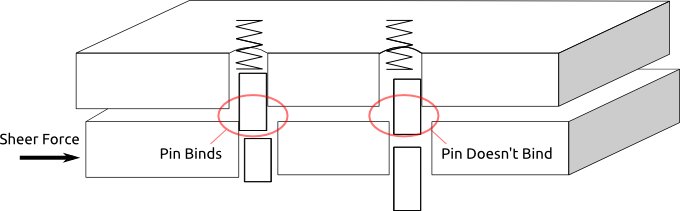
\includegraphics[width=\textwidth]{figure4.1}
    \caption{(a) Sheer force causes driver to bind}
\end{figure}

\begin{figure}
    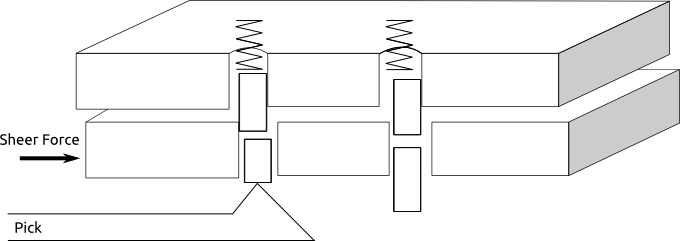
\includegraphics[width=\textwidth]{figure4.2}
    \caption{(b) Pick lifts the binding pin}
\end{figure}

\begin{figure}
    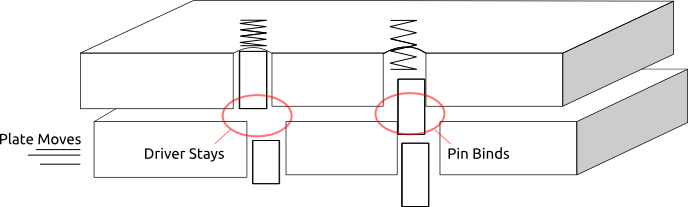
\includegraphics[width=\textwidth]{figure4.3}
    \caption{(c) Left driver sets and right driver binds}
\end{figure}
